\section{Appendix}
\label{sec:appendix}

\section{A. Muon Energies in the Detectors}

%inner detector system
\begin{table}[h]
		\centering
        \begin{tabular}{ccc}
            \toprule
             Event no. & $p_T$ [Gev/$c$] & $p$ [Gev/$c$] \\
            \midrule
            $1 $ & $-38.36 \pm 1.016$ & $-85.28$ \\
  			\midrule
  			$2 $ & $ 33.17 \pm 0.797$ & $ 43.40$ \\
  			\midrule
  			$4 $ & $ 41.96 \pm 0.831$ & $ 48.89$ \\
  			\midrule
  			$5 $ & $-53.66 \pm 2.054$ & $-168.16$ \\
  			\midrule
  			$6 $ & $ 44.65 \pm 1.388$ & $ 117.32$ \\
  			\midrule
  			$7 $ & $-57.34 \pm 1.684$ & $-71.94$ \\
  			\midrule
  			$8 $ & $ 64.54 \pm 2.677$ & $ 199.91$ \\
  			\midrule
  			$9 $ & $-55.54 \pm 1.150$ & $-57.84$ \\
  			\midrule
  			$11$ & $-37.79 \pm 1.185$ & $-100.75$ \\
  			\midrule
  			$12$ & $ 37.59 \pm 0.653$ & $ 38.26$ \\
  			\midrule
  			$13$ & $-59.88 \pm 1.766$ & $-105.19$ \\
  			\midrule
  			$15$ & $-43.88 \pm 1.471$ & $-131.69$ \\
  			\midrule
  			$16$ & $ 45.66 \pm 1.844$ & $ 152.24$ \\
  			\midrule
  			$17$ & $-32.65 \pm 0.539$ & $-35.23$ \\
  			\midrule
  			$18$ & $ 52.80 \pm 1.060$ & $ 54.19$ \\
  			\midrule
  			$19$ & $-64.49 \pm 2.515$ & $-84.75$ \\
  			\midrule
  			$20$ & $ 47.56 \pm 1.324$ & $ 104.26$ \\
  			\midrule
  			$22$ & $ 52.73 \pm 1.304$ & $ 100.36$ \\
  			\midrule
  			$23$ & $-44.56 \pm 1.470$ & $-117.21$ \\
			\bottomrule
        \end{tabular}
        \caption{Energy Loss measurement data in the Inner Detector}
        \label{tab:innerdetector}
    \end{table}
\FloatBarrier

%muon detector system
\begin{table}[h]
		\centering
        \begin{tabular}{ccc}
            \toprule
             Event no. & $p_T$ [Gev/$c$] & $p$ [Gev/$c$] \\
				\midrule
				$1 $ & $-24.06 \pm 2.579$ & $-53.92$ \\
			\midrule
			$2 $ & $ 33.35 \pm 1.675$ & $ 43.83$ \\
			\midrule
			$4 $ & $ 38.11 \pm 1.333$ & $ 44.77$ \\
			\midrule
			$5 $ & $-61.17 \pm 4.417$ & $-177.62$ \\
			\midrule
			$6 $ & $ 36.60 \pm 3.150$ & $ 96.56$ \\
			\midrule
			$7 $ & $-51.82 \pm 1.070$ & $-64.96$ \\
			\midrule
			$8 $ & $ 64.89 \pm 2.846$ & $ 199.44$ \\
			\midrule
			$9 $ & $-48.00 \pm 0.948$ & $-50.01$ \\
			\midrule
			$11$ & $-35.03 \pm 0.659$ & $-94.11$ \\
			\midrule
			$12$ & $ 33.85 \pm 1.157$ & $ 34.48$ \\
			\midrule
			$13$ & $-62.15 \pm 4.197$ & $-108.68$ \\
			\midrule
			$15$ & $-41.97 \pm 2.098$ & $-125.51$ \\
			\midrule
			$16$ & $ 47.26 \pm 2.169$ & $ 157.69$ \\
			\midrule
			$17$ & $-29.81 \pm 0.531$ & $-32.18$ \\
			\midrule
			$18$ & $ 48.73 \pm 2.261$ & $ 50.00$ \\
			\midrule
			$19$ & $-52.18 \pm 1.038$ & $-68.09$ \\
			\midrule
			$20$ & $ 49.52 \pm 3.217$ & $ 107.98$ \\
			\midrule
			$22$ & $ 53.09 \pm 8.798$ & $ 101.13$ \\
			\midrule
			$23$ & $-42.55 \pm 2.235$ & $-112.26$ \\
			\bottomrule
        \end{tabular}
        \caption{Energy Loss measurement data in the Muon Detector}
        \label{tab:muondetector}
    \end{table}
\FloatBarrier

\section{B. Muon Energies in the Detectors}
\label{sec:sectionB}

\subsubsection{Full $η$ cuts in \texttt{ElecCalib.c}}
\begin{lstlisting}
#include "math.h"
#include "TMath.h"

double ElecCalib(double e_raw, double pt, double eta,
		 double phi, double etiso, double eoverp,
		 double mindrjet)
{
  double dummy=pt*eta*phi*etiso*eoverp*mindrjet;
  double energy = e_raw;

  if  (0<fabs(eta)<0.2) energy = energy * 91.2/90.14;
  else if (0.2<fabs(eta)<0.4) energy = energy * 91.2/90.1;
  else if (0.4<fabs(eta)<0.6) energy = energy * 91.2/90.07;
  else if (0.6<fabs(eta)<0.8) energy = energy * 91.2/89.79;
  else if (0.8<fabs(eta)<1.0) energy = energy * 91.2/89.47;
  else if (1.0<fabs(eta)<1.2) energy = energy * 91.2/89.50;
  else if (1.2<fabs(eta)<1.4) energy = energy * 91.2/89.48;
  else if (1.4<fabs(eta)<1.6) energy = energy * 91.2/90.10;
  else if (1.6<fabs(eta)<1.8) energy = energy * 91.2/91.25;
  else if (1.8<fabs(eta)<2.0) energy = energy * 91.2/91.27;
  else if (2.0<fabs(eta)<2.2) energy = energy * 91.2/89.03;
  else if (2.2<fabs(eta)<2.4) energy = energy * 91.2/88.11;
  else if (2.4<fabs(eta)<2.5) energy = energy * 91.2/87.77;

  return energy;
}
\end{lstlisting}

\subsubsection{Energy and  $η$ cuts in \texttt{ElecCalib.c}}
\begin{lstlisting}
#include "math.h"
#include "TMath.h"

double ElecCalib(double e_raw, double pt, double eta,
		 double phi, double etiso, double eoverp,
		 double mindrjet)
{
  double dummy=pt*eta*phi*etiso*eoverp*mindrjet;
  double energy = e_raw;

if  (0.<fabs(eta)<0.5) {
	if (e_raw<30) energy = energy * 91.2/89.69;
	else if (30<e_raw && e_raw<40) energy = energy * 91.2/89.64;
	else if (40<e_raw && e_raw<50)  energy = energy * 91.2/90.53;
	else if (50<e_raw && e_raw<70)  energy = energy * 91.2/90.81;
	else if (e_raw > 70) energy = energy * 91.2/90.61;
}

else if (0.5<fabs(eta)<1.) {
	if (e_raw<30) energy = energy * 91.2/89.55;
	else if (30<e_raw && e_raw<40) energy = energy * 91.2/89.02;
	else if (40<e_raw && e_raw<50)  energy = energy * 91.2/89.77;
	else if (50<e_raw && e_raw<70)  energy = energy * 91.2/90.43;
	else if (e_raw > 70) energy = energy * 91.2/90.77;
}

else if (1<fabs(eta)<1.5) {
	if (e_raw<30) energy = energy * 91.2/87.49;
	else if (30<e_raw && e_raw<40) energy = energy * 91.2/88.91;
	else if (40<e_raw && e_raw<50)  energy = energy * 91.2/87.64;
	else if (50<e_raw && e_raw<70)  energy = energy * 91.2/89.37;
	else if (e_raw > 70) energy = energy * 91.2/90.37;
}

else if (1.5<fabs(eta)<2.) {
	if (e_raw<80) energy = energy * 91.2/89.81;
	else if (80<e_raw && e_raw<180) energy = energy * 91.2/91.35;
	else if (e_raw > 70) energy = energy * 91.2/91.76;
}


else if (2.<fabs(eta)<2.5)   {
	if (e_raw<150) energy = energy * 91.2/88.53;
	else if (e_raw > 150) energy = energy * 91.2/88.87;
}
  return energy;
}
\end{lstlisting}

\subsubsection{Coarse $η$ cuts in \texttt{ElecCalib.c}}
\begin{lstlisting}
#include "math.h"
#include "TMath.h"

double ElecCalib(double e_raw, double pt, double eta,
		 double phi, double etiso, double eoverp,
		 double mindrjet)
{
  double dummy=pt*eta*phi*etiso*eoverp*mindrjet;
  double energy = e_raw;
	if  (0.<fabs(eta)<0.5) energy = energy * 91.2/90.18;
    else if (0.5<fabs(eta)<1.) energy = energy * 91.2/90.12;
    else if (1<fabs(eta)<1.5) energy = energy * 91.2/89.8;
    else if (1.5<fabs(eta)<2.) energy = energy * 91.2/91.22;
    else if (2.<fabs(eta)<2.5) energy = energy * 91.2/88.72;
  return energy;
}
\end{lstlisting}

\section{W-mass}

\begin{figure}
    \begin{subfigure}{0.5\textwidth}
        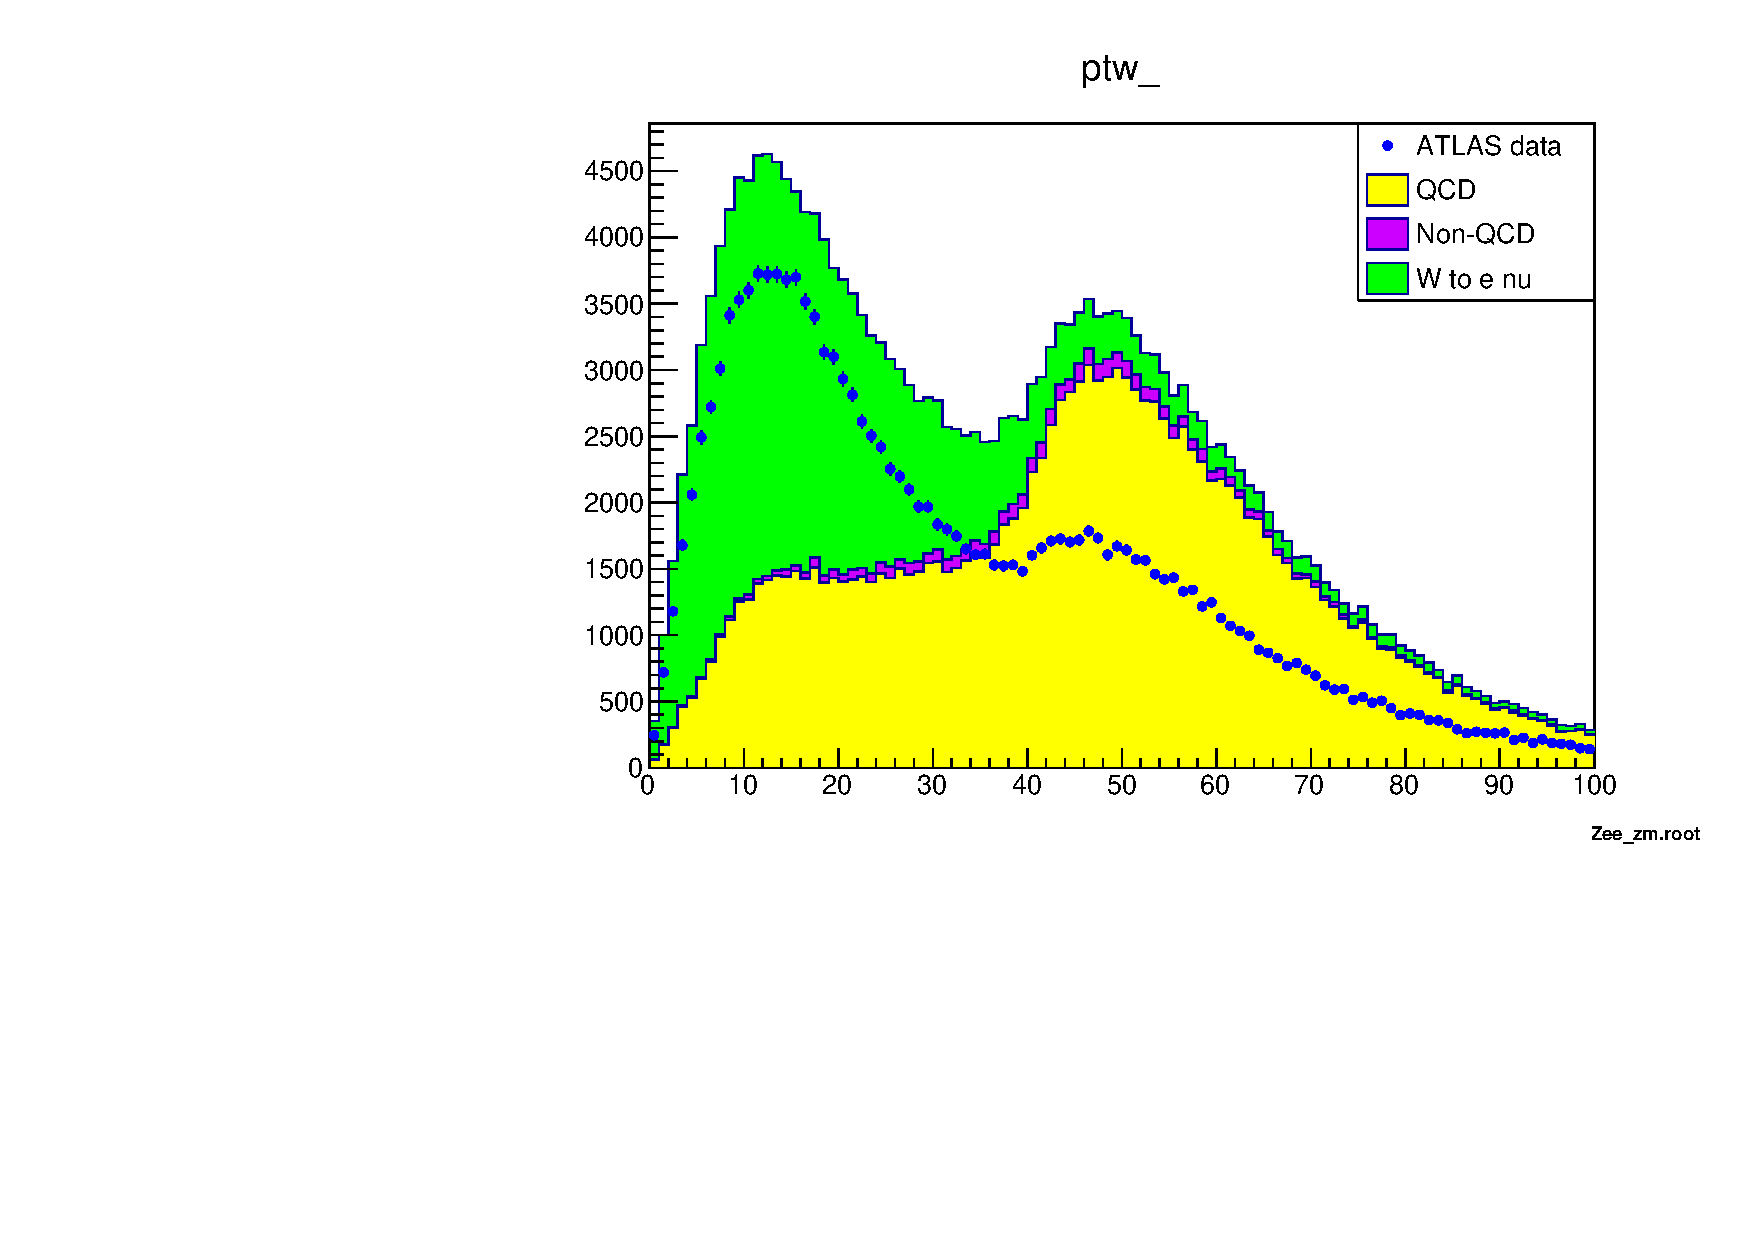
\includegraphics[width=\textwidth]{../W_mass/ptw_100_0_100_qcd1.pdf}
    \end{subfigure}
    \begin{subfigure}{0.5\textwidth}
        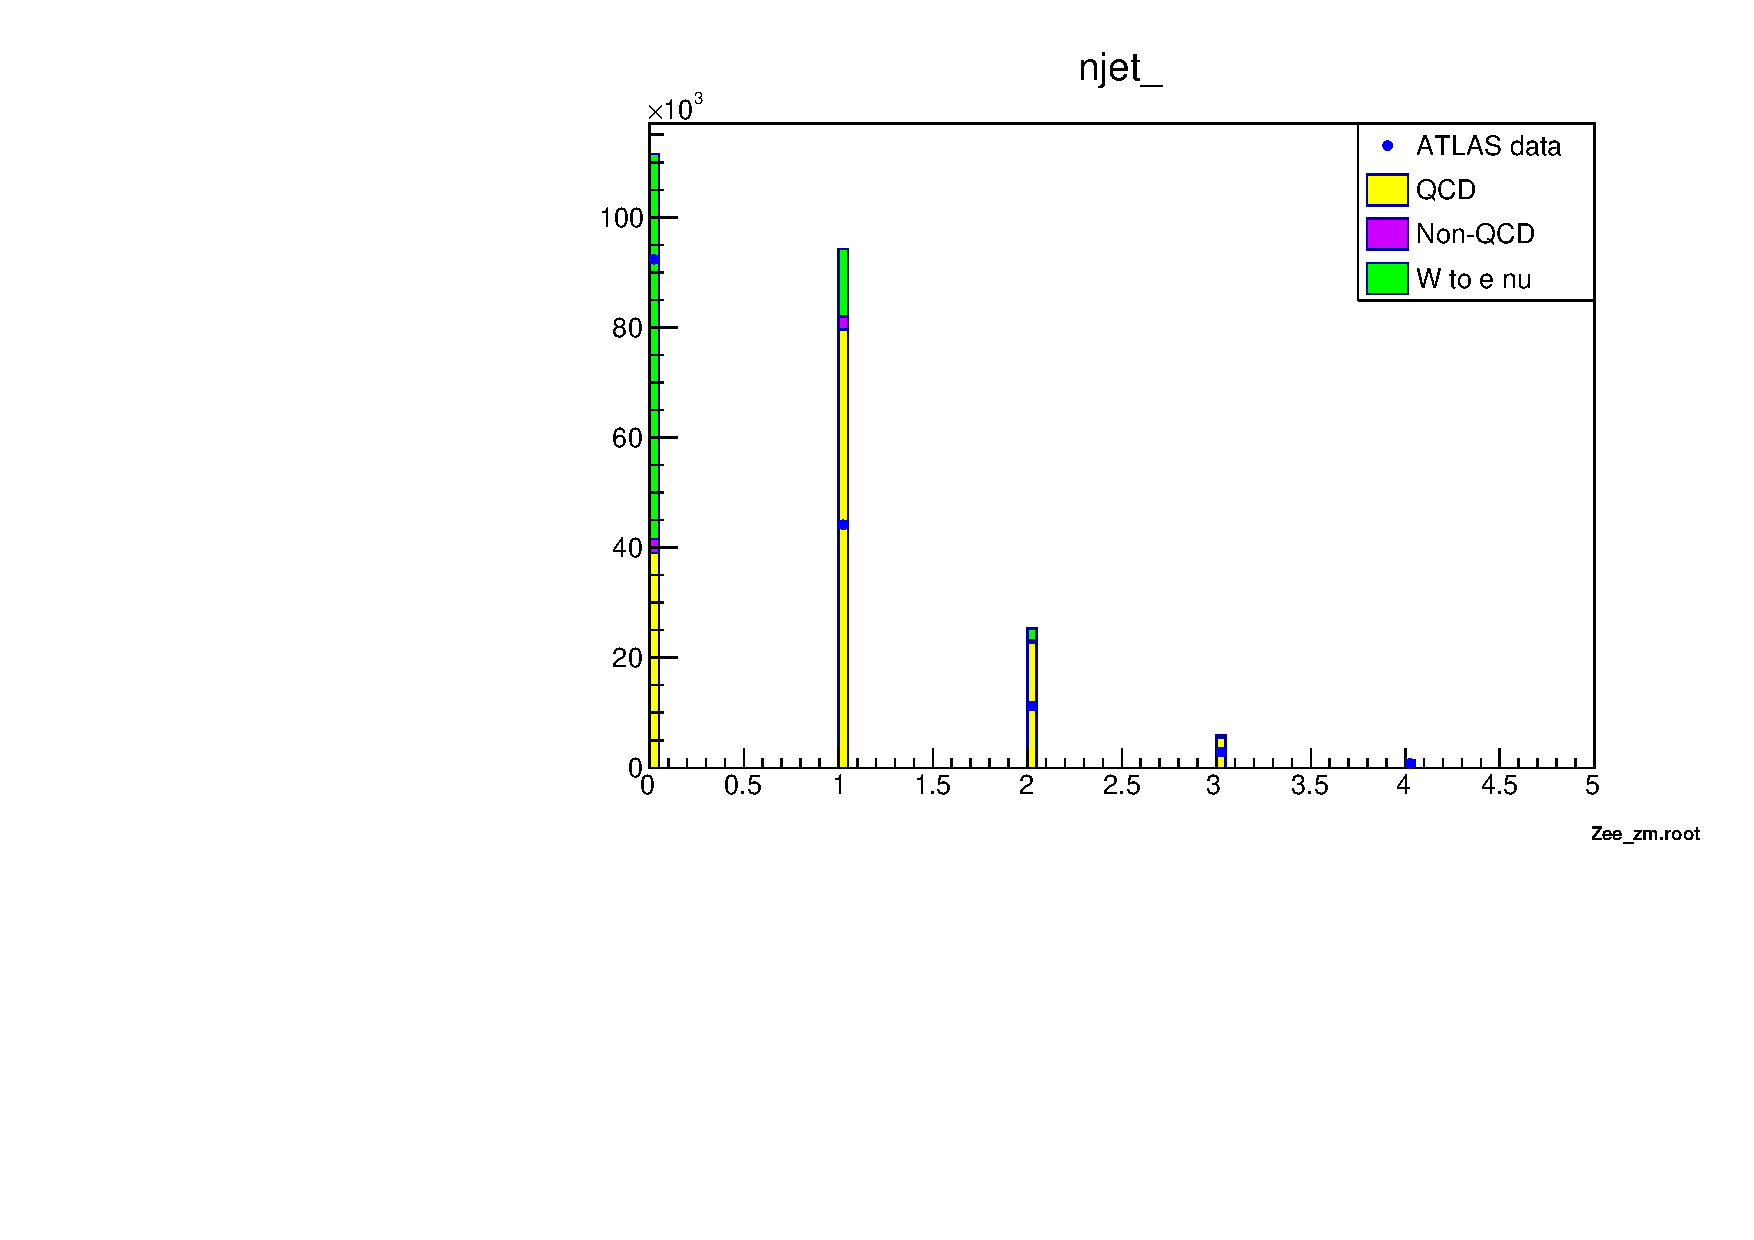
\includegraphics[width=\textwidth]{../W_mass/njet_100_0_5_qcd1.pdf}
    \end{subfigure}
    \begin{subfigure}{0.5\textwidth}
        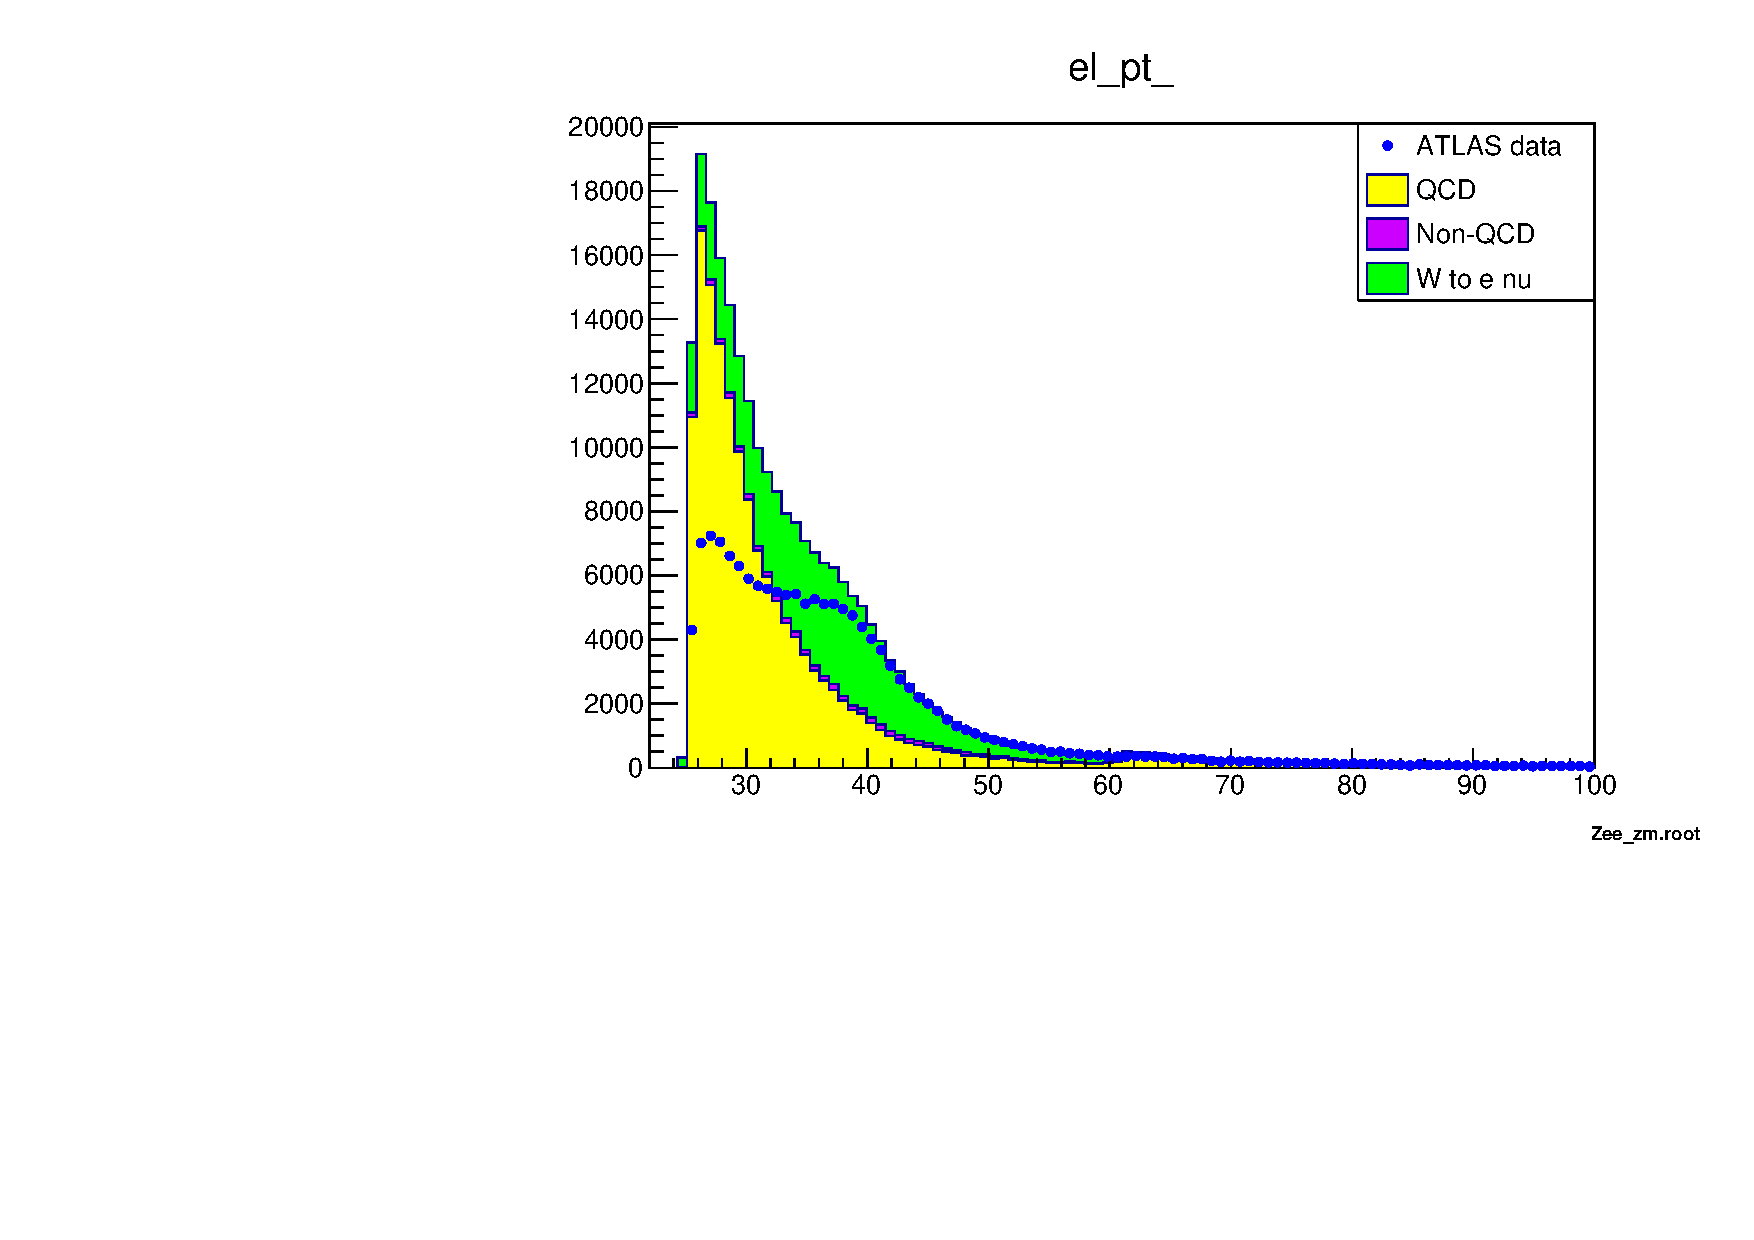
\includegraphics[width=\textwidth]{../W_mass/elpt_100_25_100_qcd1.pdf}
    \end{subfigure}
    \begin{subfigure}{0.5\textwidth}
        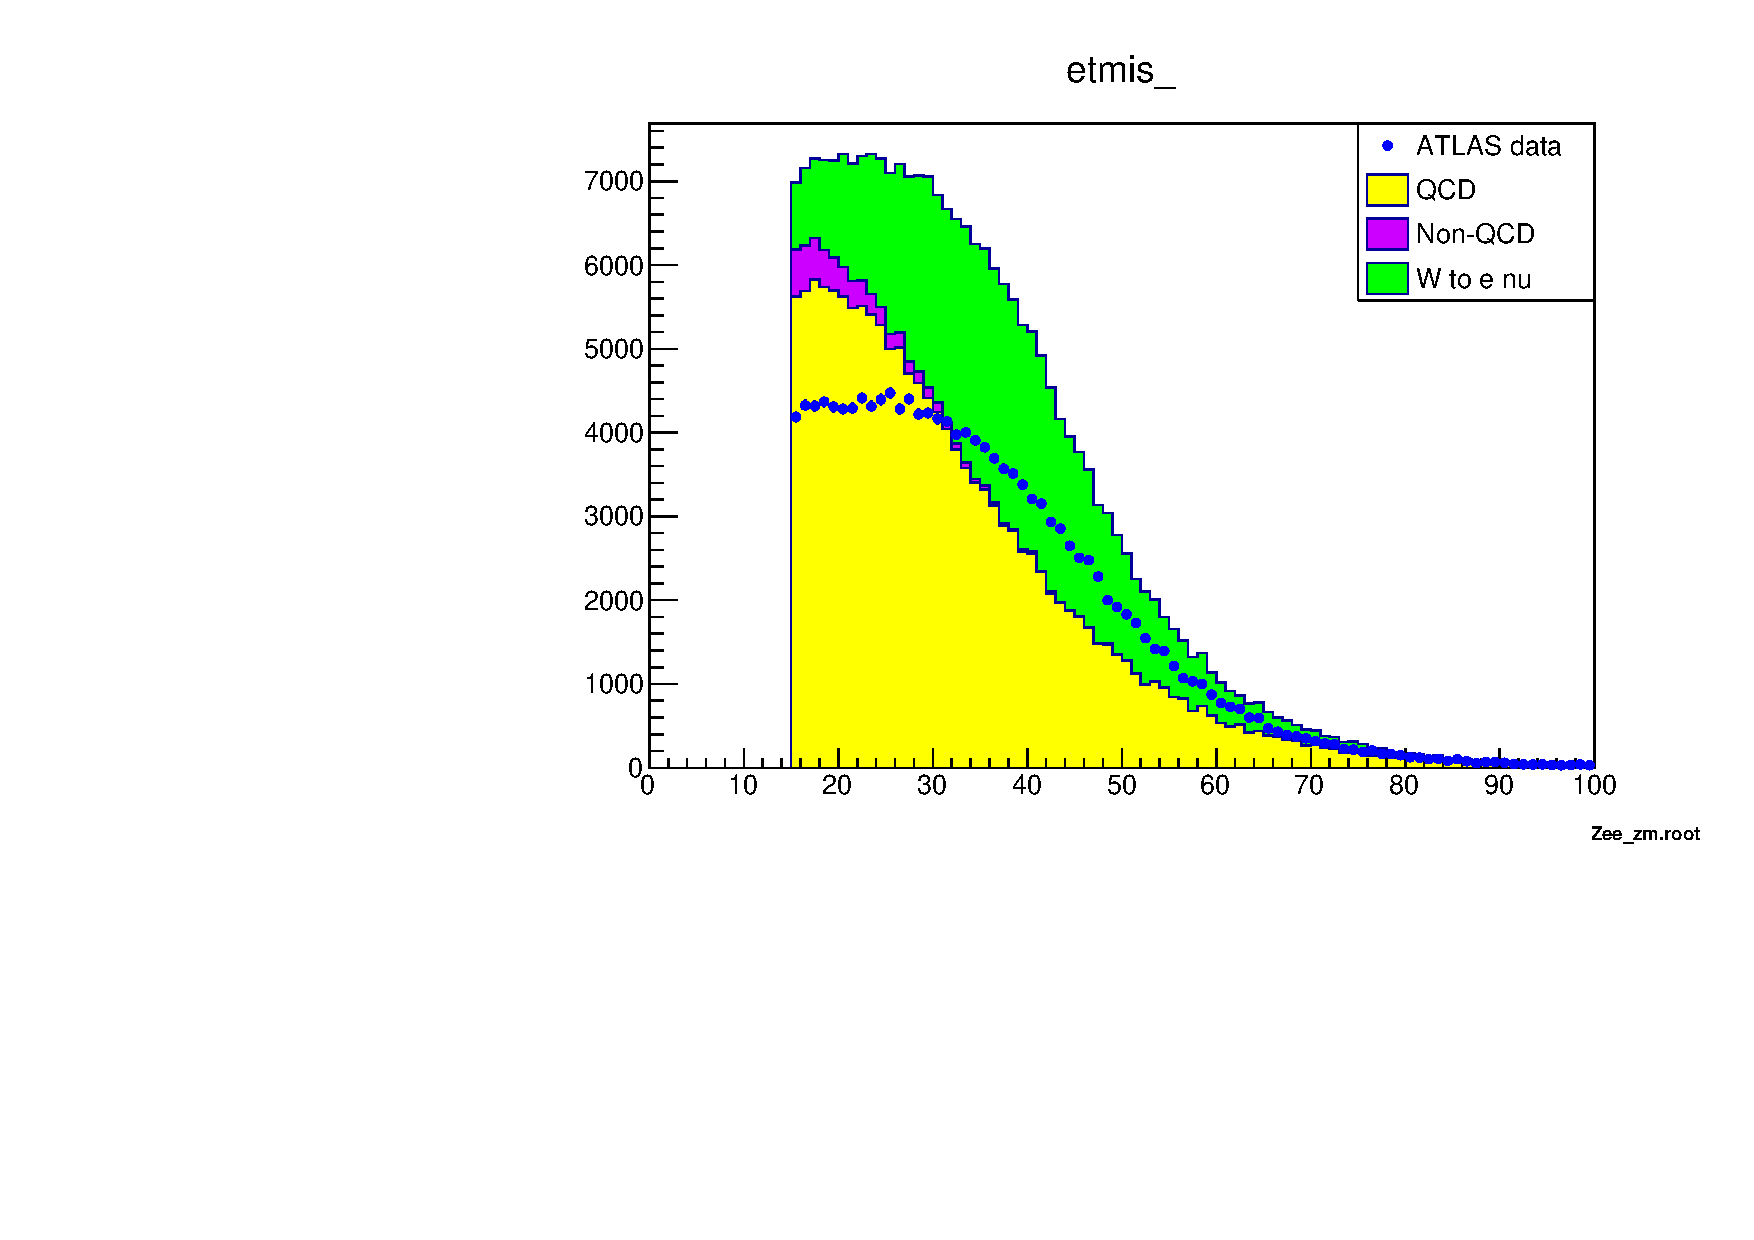
\includegraphics[width=\textwidth]{../W_mass/etmis_100_0_100_qcd1.pdf}
    \end{subfigure}
    \caption{Distributions of the kinematic variables \texttt{ptw, njet, el\_pt} and \texttt{etmis} for a QCD scale factor of 1}
    \label{fig:qcd1}
\end{figure}

\begin{figure}
    \centering
    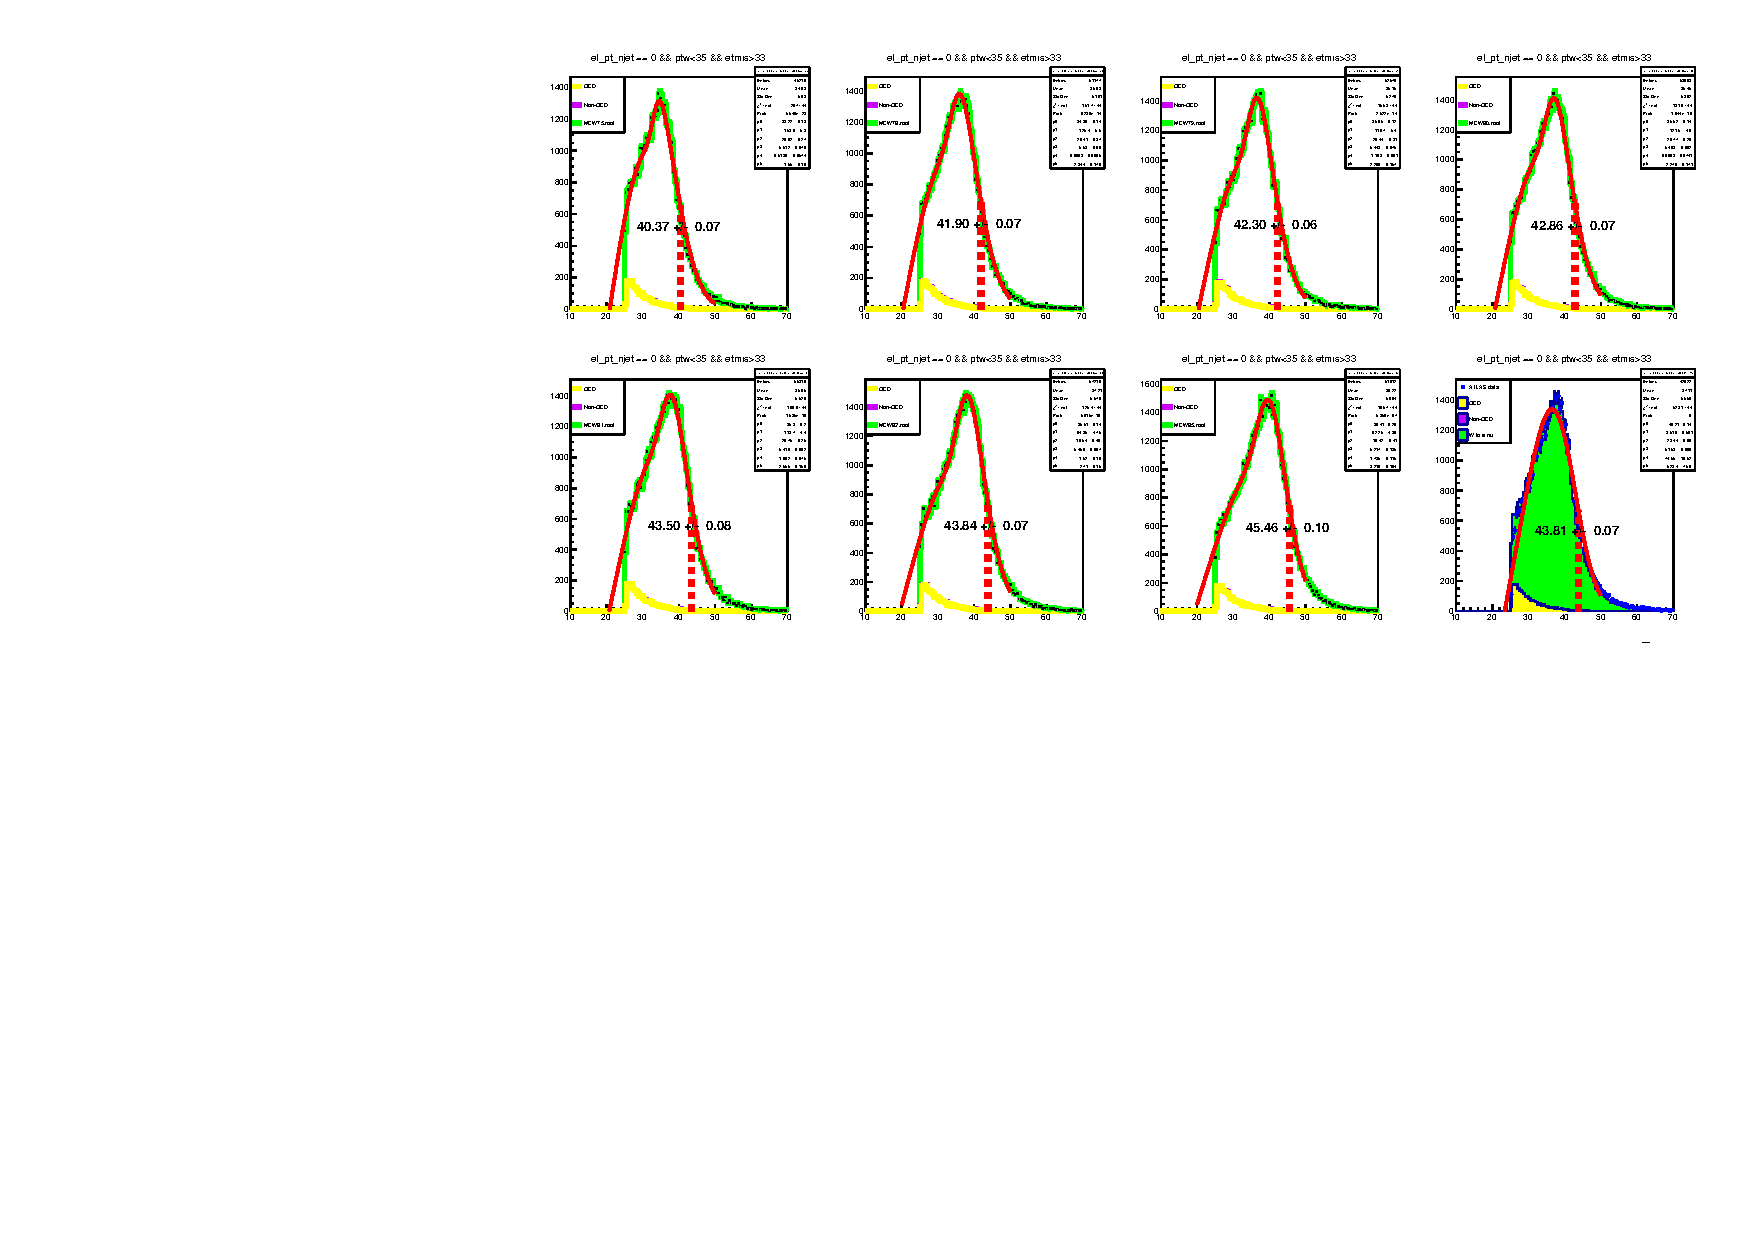
\includegraphics[width=0.8\textwidth]{../W_mass/gauge_curve_cuts1.pdf}
    \caption{Fits to the Jacobi peak in the electron transverse momentum spectrum for different
    W masses.}
    \label{fig:gauge_curve_cuts1}
\end{figure}



\begin{figure}
    \centering
    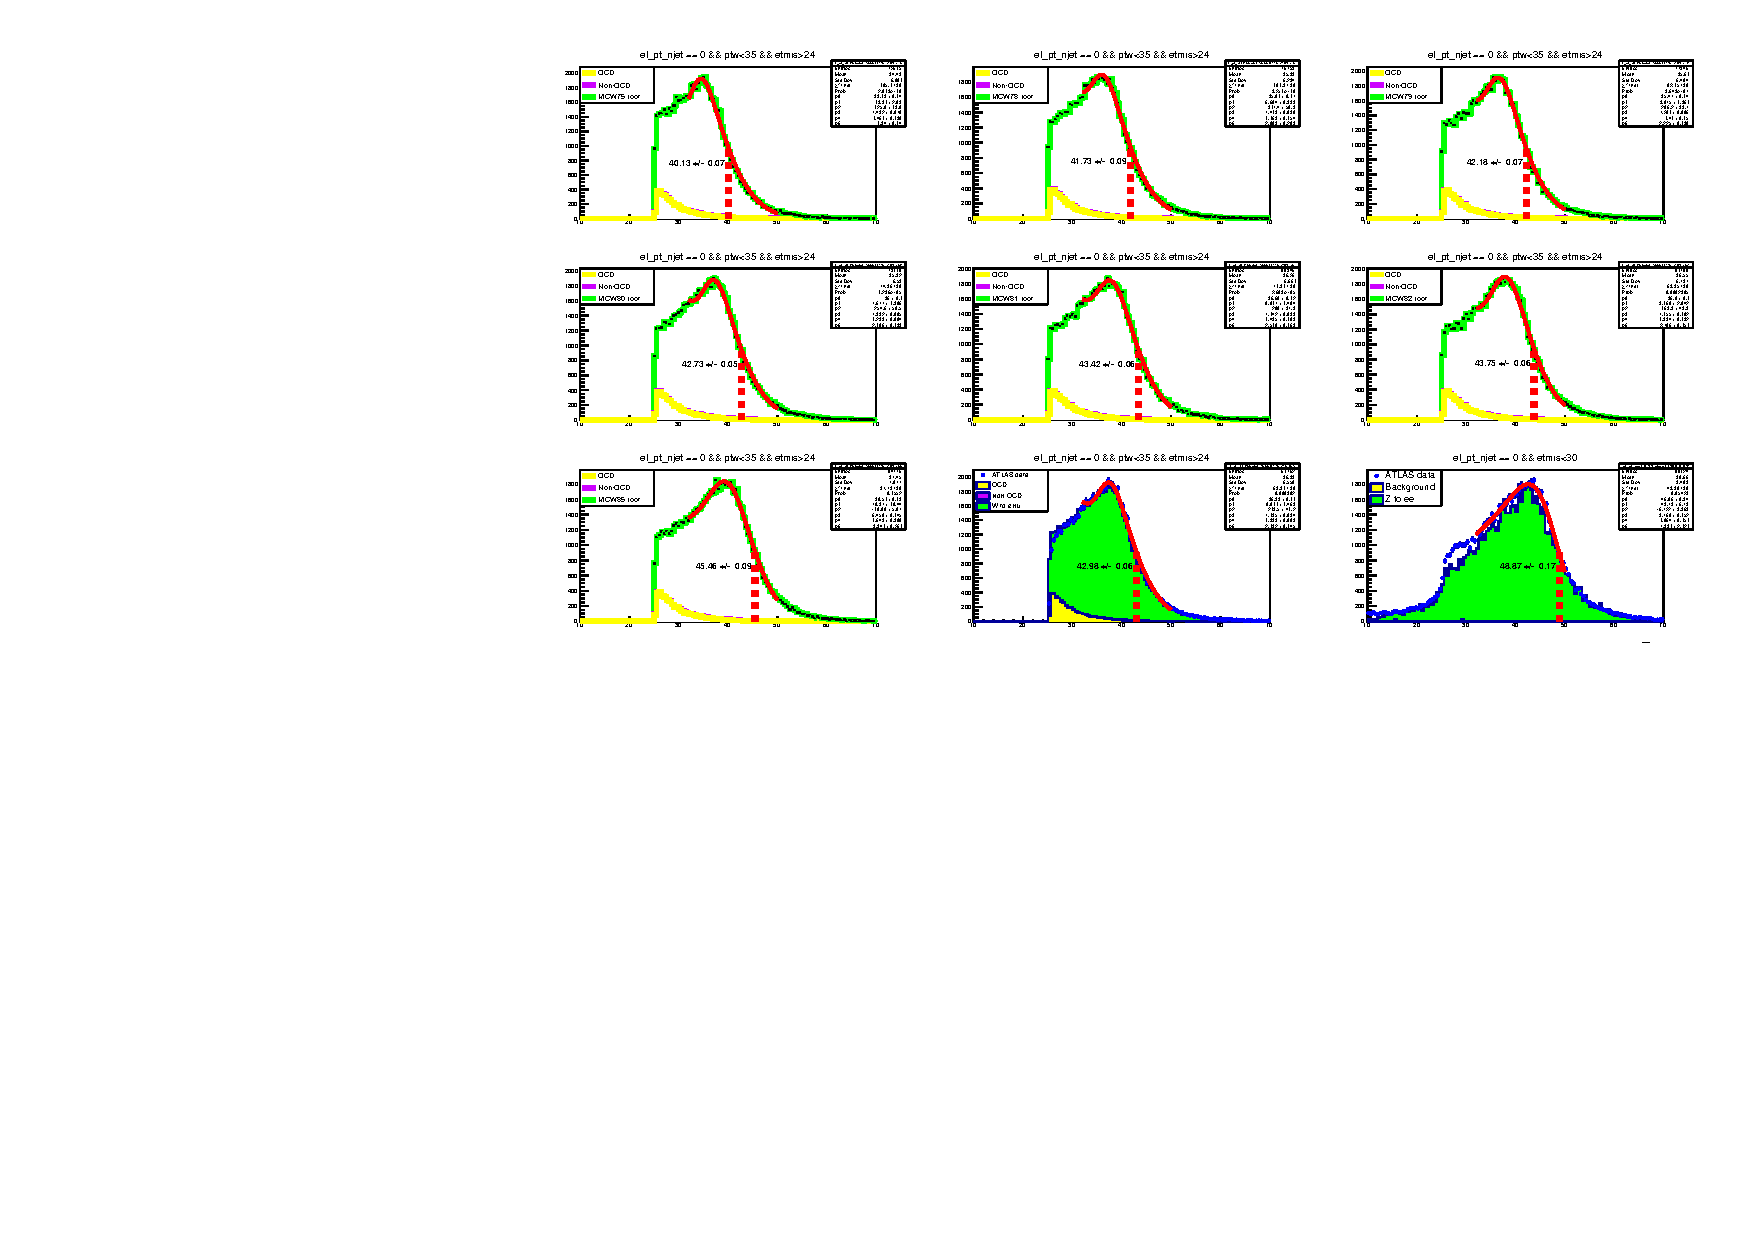
\includegraphics[width=0.8\textwidth]{../W_mass/gauge_curve_etmis24.pdf}
    \caption{Fits to the Jacobi peak in the electron transverse momentum spectrum for the final set of cuts \texttt{njet == 0 \&\& ptw < 35 \&\& etmis > 24}.}
    \label{fig:Jacobi-final}
\end{figure}

\begin{figure}
    \centering
    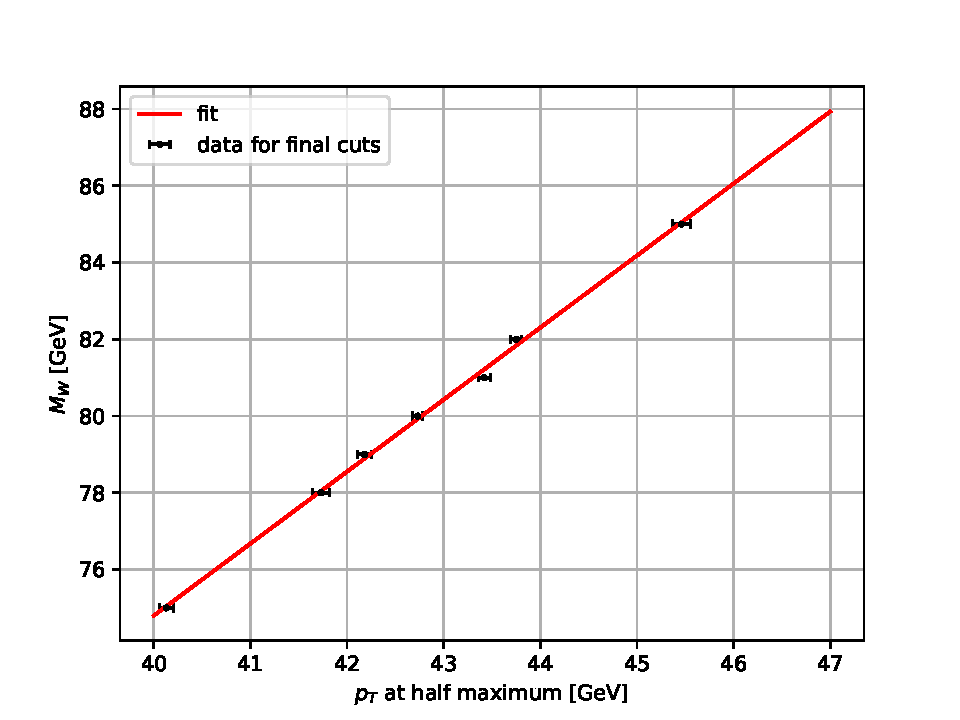
\includegraphics[width=0.8\textwidth]{../W_mass/final_gauge_curv.pdf}
    \caption{Gauge curve for final set of cuts \texttt{njet == 0 \&\& ptw < 35 \&\& etmis > 24}.}
    \label{fig:gauge_final}
\end{figure}